\documentclass[11pt]{article}

\usepackage{verbatim}
\usepackage{amsmath}
\usepackage{amssymb}
\usepackage{setspace}
\usepackage[top=1in, bottom=1in, left=1.25in, right=1.25in]{geometry}
\usepackage{subfigure}
\usepackage{graphicx}
\usepackage{cite}
\usepackage[squaren]{SIunits}
\usepackage{listings}
\usepackage{csquotes}

\setlength{\parindent}{0pt} 	% remove the silly paragraph indents

% Sample figure
%\begin{figure}[h!]
%\centering
%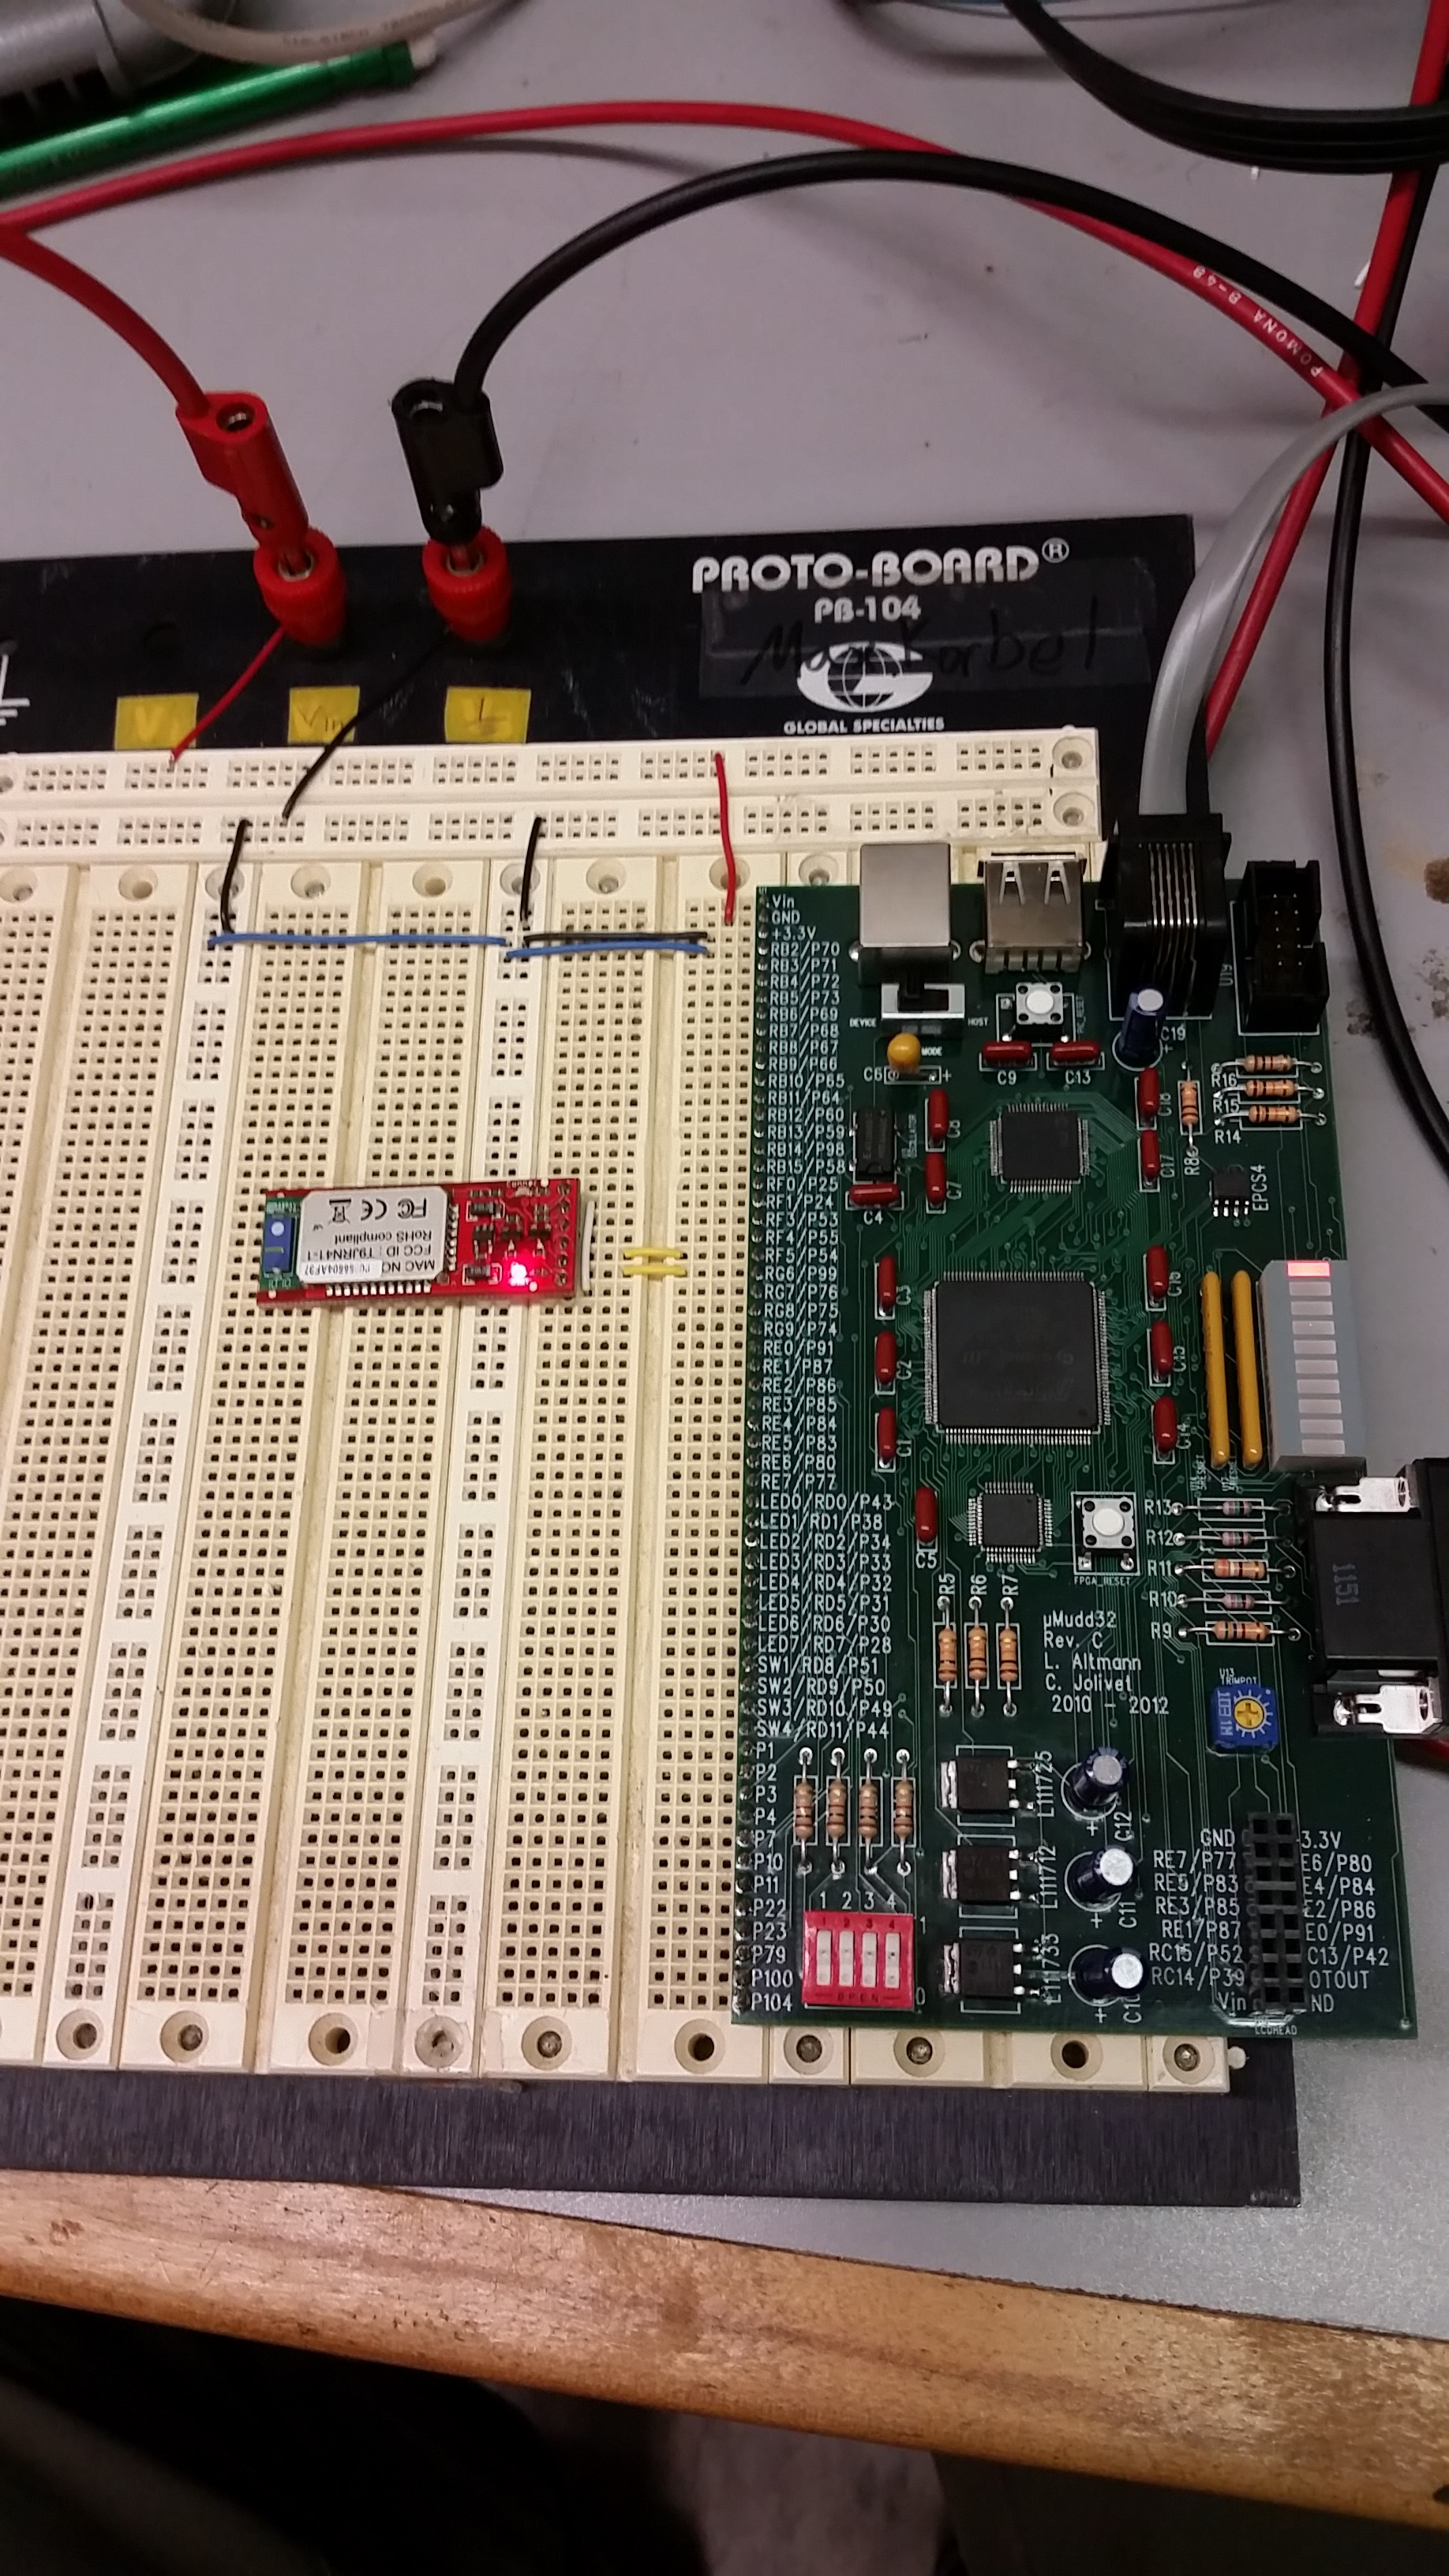
\includegraphics[scale=0.11]{board.jpg}
%\caption{The latest number entered on the keypad is displayed on the bottom display. The second latest number is displayed on the top.}
%\label{fig:board}
%\end{figure} 


\begin{document}



% ---------------------------------------
% Name section
% ---------------------------------------
\begin{flushleft}
Sherman Lam
\\E155
\\ \today
\end{flushleft}


% ---------------------------------------
% Title
% ---------------------------------------
\begin{center}
\begin{Large}
\textbf{Lab 6 Report: Wireless Calculator}
\end{Large}
\end{center}


% ---------------------------------------
% Start report
% ---------------------------------------


\section{Introduction}

In this lab, I built a wireless calculator using a PIC32 microcontroller and a bluetooth module. The module used was the Sparkfun BlueSMiRF. The PIC interfaces with the BlueSMiRF through UART. On the other end of the bluetooth link is a generic USB bluetooth module connected to my laptop. I send mathematical expressions over the bluetooth link through a PuTTY terminal.

\begin{figure}[h!]
\centering
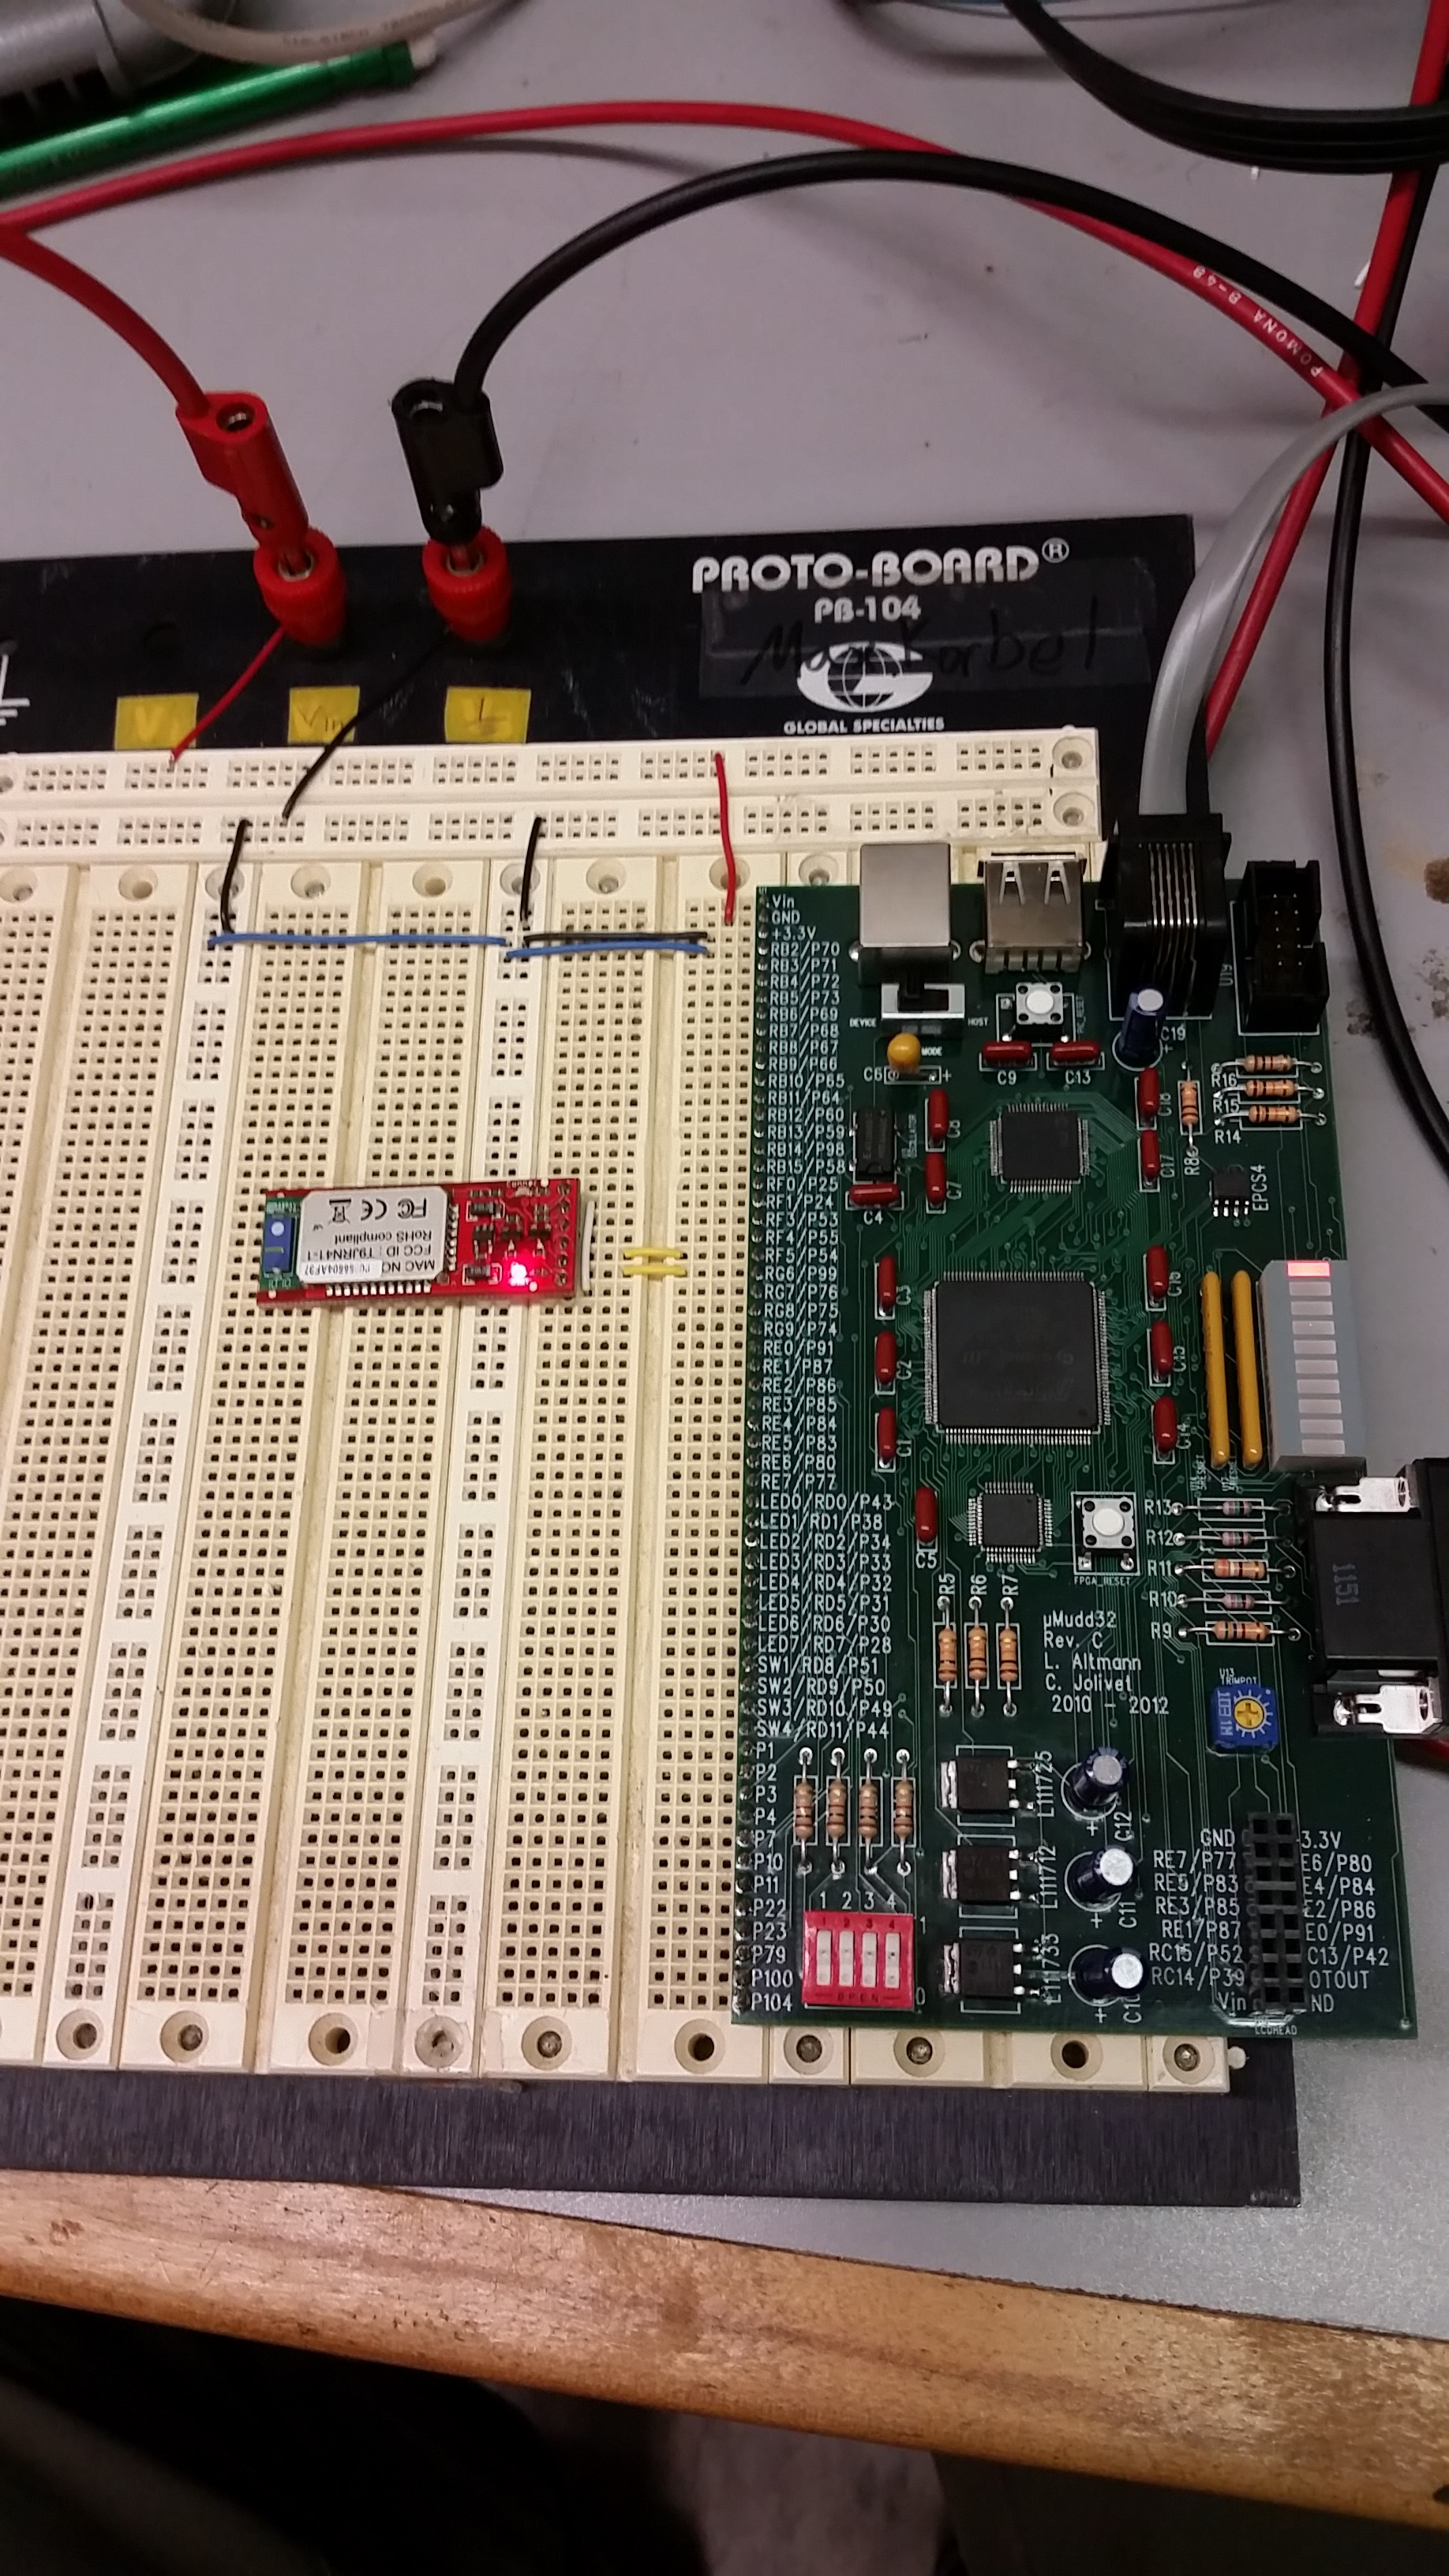
\includegraphics[scale=0.11]{board.jpg}
\caption{The latest number entered on the keypad is displayed on the bottom display. The second latest number is displayed on the top.}
\label{fig:board}
\end{figure} 


\section{Design and Testing Methodology}

\subsection{Algorithm}

When strings are received, they contain a wide variety of chars. This includes numbers, mathematical symbols, and string modification characters (e.g. delete, new line, and carriage return). To correctly interpret the input string, I first ``clean" the string by removing all white spaces, new lines, and carriage returns. I then modify the string to account for backspaces. If the input was a valid mathematical expression, the final cleaned expression is of form A(B)C where (B) is an operator. The expression can then be parsed and evaluated in a consistent manner. The operations handled in this calculator are summation (+), subtraction (-), multiplication (*), and integer division (/).


\subsection{Hardware}
There were no special hardware connections needed. The BlueSMiRF was powered from 3.3V. The CTS and RTS pins on the BlueSMiRF were connected together as instructed by the lab. The TX pin on the BlueSMiRF was connected to the RX pin of the PIC's UART2 (RF4). The RX pin on the BlueSMiRF was connected to the TX pin of the PIC's UART22 (RF5). 
	

\subsection{UART}

The PIC communicates with the BlueSMiRF through UART2. May computer communicates with the bluetooth dongle through a serial connection. The communication protocols used in each are defined as follows: \\

\textbf{PIC-BlueSMiRF protocol:}
\begin{description}
	\item[Speed: ] 115.2k baud
	\item[Data bits: ] 8
	\item[Stop bits: ] 1
	\item[Parity: ] none
	\item[Flow control: ] none \\
\end{description}

\textbf{Bluetooth Dongle - Computer protocol:}
\begin{description}
	\item[Speed: ] 9600 baud
	\item[Data bits: ] 8
	\item[Stop bits: ] 1
	\item[Parity: ] none
	\item[Flow control: ] none \\
\end{description}

When programming the PIC, one of the registers that must be set is the U2BRG. This register controls the baud rate of the UART connection. The BRG is calculated by the following:

\begin{align*}
f_{UART} &= \frac{f_{peripheral-clock}}{16(BRG+1)} \\
BRG &= \frac{f_{peripheral-clock}}{16f_{UART}}-1
\end{align*}

So, for a baud rate ($f_{UART}$) of 115.2kHz and a peripheral clock of $20MHz$, the desired value of BRG is:

\begin{align*}
BRG &= \frac{f_{peripheral-clock}}{16f_{UART}}-1 \\
	&= \frac{20MHz}{16*115.2kHz}-1 \\
	& \approx 10
\end{align*}

\subsection{Test Cases}
Each of the supported operations where tested. Various incomplete expressions were also tested to check for error handling. The program executes the operations correctly and prints an error statement when asked to evaluate invalid or incomplete expressions. The following is a subset of the test cases used as well as their corresponding outputs. \\

You typed: 132+456 \\
Answer: 588 \\

You typed: 789-123 \\
Answer: 666 \\

You typed: 5-6 \\
Answer: -1 \\

You typed: 7*6 \\
Answer: 42 \\

You typed: 6/4 \\
Answer: 1 \\

You typed: 14/0 \\
Cannot divide by 0 \\

You typed: 0/456 \\
Answer: 0 \\

You typed: 1+ \\
Incomplete equation \\

You typed: sdfg \\
Equation invalid \\

You typed: 123+abc \\ 
Equation invalid \\


\section{Technical Documentation}

This section provides the C-code used to program the PIC.

\subsection{C code}

\begin{lstlisting}[numbers=left,language=C,basicstyle=\footnotesize]
#include <stdio.h>
#include <P32xxxx.h>

/* Functions prototypes */
void initMODE(void);
void initSTA(void);
void initBRG(void);
char getcharserial(void);
void getstrserial(char*);
void sendcharserial(char);
void sendstrserial(char*);
void clean(char*, char*);
void parse(char*);
int isNum(char);
int isOp(char);
void domath(int, int, char);


/*
This inits UART control register values.

Author: Sherman Lam
Email: slam@g.hmc.edu
Date: 10-16-14
*/
void initUART(void){
    // set I/O pins
    TRISFbits.TRISF5 = 0;
    TRISFbits.TRISF4 = 1;
    
    //call all the individual init functions
    initMODE();
    initSTA();
    initBRG();
}


/* 
This inits the control register U2MODE. From lecture slides.

bit 31-16: unused
bit 15: ON = 1: enable UART
bit 14: FRZ = 0: don't care when CPU in normal state
bit 13: SIDL = 0: don't care when CPU in normal state
bit 12: IREN = 0: disable IrDA
bit 11: RTSMD = 0: don't care if not using flow control
bit 10: unused
bit 9-8: UEN = 00: enable U1TX and U1RX, disable U1CTSb and U1RTSb
bit 7: WAKE = 0: do not wake on UART if in sleep mode
bit 6: LPBACK = 0: disable loopback mode
bit 5: ABAUD = 0: don't auto detect baud rate
bit 4: RXINV = 0: U1RX idle state is high
bit 3: BRGH = 0: standard speed mode
bit 2-1: PDSEL = 00: 8-bit data, no parity
bit 0: STSEL = 0: 1 stop bit

Author: Sherman Lam
Email: slam@g.hmc.edu
Date: 10-16-14
*/
void initMODE(void){
    U2MODE = 0x8000;
}


/*
This inits the control register U2STA. From lecture slides.

bit 31-25: unused
bit 24-16: write 0 when not using auto address detect
bit 15-14: UTXISEL = 00: interrupt when TX buffer not full
bit 13: UTXINV = 0: U1TX idle state is high
bit 12: URXEN = 1: enable receiver
bit 11: UTXBRK = 0: disable break transmission
bit 10: UTXEN = 1: enable transmitter
bit 9: UTXBF: don't care (read-only)
bit 8: TRMT: don't care (read-only)
bit 7-6: URXISEL = 00: interrupt when receive buffer not empty
bit 5: ADDEN = 0: disable address detect
bit 4: RIDLE: don't care (read-only)
bit 3: PERR: don't care (read-only)
bit 2: FERR: don't care (read-only)
bit 1: OERR = 0: reset receive buffer overflow flag
bit 0: URXDA: don't care (read-only)

Author: Sherman Lam
Email: slam@g.hmc.edu
Date: 10-16-14
*/
void initSTA(void){ 
    U2STA = 0x1400;
}


/*
This inits the control register BRG. From lecture slides.

Want rate of 115.2 Kbaud
Assuming PIC peripheral clock Fpb = Fosc / 2 = 20 MHz
based on default instructions in lab 1.
U3BRG = (Fpb / 4*baud rate) - 1
-> U3BRG = 10 (decimal)
Actual baud rate 113636.4 (-1.2% error)

Author: Sherman Lam
Email: slam@g.hmc.edu
Date: 10-16-14
*/
void initBRG(void){
    U2BRG = 10;
}


/*
This waits until there is a char available from the serial port and returns it

Author: Sherman Lam
Email: slam@g.hmc.edu
Date: 10-23-14
*/
char getcharserial(void){
    //wait for data to be available
        //printf("Reading serial\n");
    while(!(U2STA & 0x1)){}

    //return char
    return U2RXREG;
}


/* This reads a string from serial

Author: Sherman Lam
Email: slam@g.hmc.edu
Date: 10-23-14
*/
void getstrserial(char* str){
    int i = 0;
    do {                            // read an entire string until detecting
        str[i] = getcharserial();   // carriage return
    } while (str[i++] != '\r');     // look for carraige return
    str[i-1] = 0;                   // null-terminate the string
}


/* This writes a single char to the tx register

Author: Sherman Lam
Email: slam@g.hmc.edu
Date: 10-23-14
*/
void sendcharserial(char data){
    //wait until the transmit buffer has space
    while(U2STA & 0x200){}          // if bit 9 = 1 -> buffer full

    //write to buffer
    U2TXREG = data;
}


/* This writes a string to the tx register

Author: Sherman Lam
Email: slam@g.hmc.edu
Date: 10-23-14
*/
void sendstrserial(char* str){
    //first send a newline and carriage return symbol to start 
    //at the beginning of a new line
    sendcharserial('\n');
    sendcharserial('\r');

    //send the str
    int i = 0;
    while(str[i] != 0){
        sendcharserial(str[i]);
        i++;
    }
}

/* This method checks is the char is number
 *
 * Author: Sherman Lam
 * Email: slam@g.hmc.edu
 * Date: 10-24-14
 */


/* This method cleans the string of new line chars, spaces, etc
 *
 * Author: Sherman Lam
 * Email: slam@g.hmc.edu
 * Date: 10-24-14
 */
void clean(char* input, char* output){
    char c = '0';
    int i = 0;      // index for iterating through input
    int j = 0;      // index for iterating through output
    do{
        c = input[i];
        if (c == ' '){}             //check if char is whitespace.
        else if ((int)c == 127){    // check backspace
            j--;                    // decrement index to overwrite last value
            if (j<0){
                j=0;
            }
        }
        else{                       // if good, write
            output[j] = c;
            j++;
        }
        i++;
    } while (c != 0);               // break if we see null terminator

    //write null terminator
    output[j] = 0;
    
}


/* This method checks if the input char is a number
 between 0 and 9

 Author: Sherman Lam
 Email: slam@g.hmc.edu
 Date: 10-25-14
 */
int isNum(char c){
    return ((48<=c) && (c<=57));        // check ascii bounds
}


/* This method checks if the input char is a valid operator

 Author: Sherman Lam
 Email: slam@g.hmc.edu
 Date: 10-25-14
 */
int isOp(char c){
    int state = 0;
    //check all supported operators
    state |= (c=='+');
    state |= (c=='-');
    state |= (c=='*');
    state |= (c=='/');
    return state;
}


/* This method does math given two integers and an operator

 Name: Sherman Lam
 Email: slam@g.hmc.edu
 Date: 10-25-14
 */
void domath(int a1, int a2, char op){
    int answer = 0;
    if (op == 43){           // +
        answer = a1 + a2;
    }
    else if (op == 45){      // -
        answer = a1 - a2;
    }
    else if (op == 42){      // *
        answer = a1 * a2;
    }
    else if (op == 47){      // /
        if (a2==0){
            printf("Cannot divide by 0 \n");
            return;
        }
        answer = a1 / a2;
    }
    else{
        printf("Operation: %c is not supported.\n\r");
        return;
    }

    printf("Answer: %d \n",answer);
}



/*
 This method parses the string and chooses which operation to perform

 Author: Sherman Lam
 Email: slam@g.hmc.edu
 Date: 10-24-14
 */
void parse(char* str){
    int i = 0;          // for indexing through string
    char c;             // a char
    int a1 = 0;         // number argument 1
    int a2 = 0;         // number argument 2
    char op = 0;        // operator
    int update1 = 0;    // whether a1 was set
    int update2 = 0;    // whether a2 was set
    //get the first number
    do{
        c = str[i];
        if (isNum(c)){
            a1 += a1*10+(c-48);
            update1 = 1;
        }
        //throw an error if a number was not entered
        else if (!isOp(c)){
            printf("Equation invalid \n");
            return;
        }
        i++;
    } while(isNum(c));  // check for number

    //get the operator
    op = c;

    //get the second number
    do{
        c = str[i];
        if (isNum(c)){
            a2 += a2*10+(c-48);
            update2 = 1;
        }
        //throw an error if a number was not entered
        else if (!(c==0)){
            printf("Equation invalid \n");
            return;
        }
        i++;
    } while(c != 0);  // check for null terminator

    // if we have all the variables, do the math. Else, print error
    if(update1 && update2){
        domath(a1,a2,op);
    }
    else{
        printf("Incomplete equation \n");
    }
}


/*
This is the main loop for interfacing with the calculator

Author: Sherman Lam
Email: slam@g.hmc.edu
Date: 10-16-14
*/
void main(void){
    // initialize the UART communiations
    initUART();

    //loop
    while(1){
            //prompt the user for an equation
            sendstrserial("Please enter an equation \n\r");

            //read the string
            char str[80];
            getstrserial(str);
            printf("\rYou typed: %s\n\r", str);

            //clean and parse the string
            char str1[80];
            clean(str,str1);
            parse(str1);
        }
}

\end{lstlisting}


\section{Results and Discussion}

The calculator performs as expected. One of the problems I was unable to fix in time is associated with the printing of backspaces. If I enter in an expression that consists only of backspaces, the output line that states ``You typed: ..." will be truncated to something along the lines of ``You ty ". However, this does not affect the printing of the answer. \\

Also note that the backspace key does not correspond with the backspace ASCII code 8. Instead, it corresponds with the delete code 127.


\section{Conclusion}

\subsection{Time Spent}

\begin{description}
	\item[Programming] 6 hrs
 	\item[Writing Report] 2hrs
	\item[Total Time Spent] 8hrs
\end{description}

\subsection{Suggestions for lab}

No suggestions for the lab.

\end{document}

